\chapter{Background}
\label{chap:background}

This dissertation investigates how children figure out the clause types of their language, on the basis of their input. In this chapter, I review what we already know from the existing literature on (1) the target knowledge, namely the formal properties of clause types and speech acts and their analyses in the formal literature; (2) children's understanding of clause types and speech acts, and the linguistic and pragmatic capacities that they can draw from early in development, and what we know about the kinds of speech acts and clause types children are exposed to. I will come back to English and Mandarin-acquiring children's morpho-syntactic knowledge in Chapter~\ref{chap:eng-cl} and Chapter~\ref{chap:man-cl}.

\section{Theories of clause types, sentential force, and speech acts} \label{sec:bg:theory}


\subsection{Speech acts and force} \label{sec:bg:theory:speech}

Frege observes that it is possible to express a thought without judging it to be true -- that considering a particular claim and judging it to be true are different things altogether. In asking a polar question like \tit{Is it raining?} one is not judging anything to be true. But in answering \tit{Yes }or asserting the declarative sentence like \tit{It is raining}, one does. Nevertheless, \tit{Is it raining?} and \tit{It is raining} have something in common: they have the same content, or as Frege puts it, they contain the same \tit{thought}. From this observation, he derives the influential distinction between \tit{content} and \tit{force}. The following passage from \tit{Der Gedanke} makes this distinction clear:

\begin{quote}
    

An interrogative sentence and an assertoric one contain the same thought; but the assertoric sentence contains something else as well, namely assertion. The interrogative sentence contains something more too, namely a request. Therefore two things must be distinguished in an assertoric sentence: the content, which it has in common with the corresponding propositional question; and assertion. The former is the thought or at least contains the thought. So it is possible to express a thought without laying it down as true. The two things are so closely joined in an assertoric sentence that it is easy to overlook their separability. 

$\,$\hfill \cite[62]{frege1918thought}, Translated by Peter Geach and R. H. Stoothoff
\end{quote}

That is, the polar question \tit{Is it raining?} and the assertion \tit{It is raining} both contain the same thought, namely \tit{whether it is raining.}  But \tit{Is it raining?} presents this thought with questioning force and \tit{It is raining} presents it with assertoric force. By presenting a thought with assertoric force, one expresses that one judges the thought to be true. But there are other ways of presenting the same thought, for example with questioning force.\footnote{However, Frege argues that the question of truth does not arise for sentences expressing commands, requests, wishes etc., so even though a sentence expressing request have sense, its sense is not a \tit{thought}.}

The idea of ``force'' is further developed by \textcite{austin1975things} in his work on speech acts. The core observation is that, utterances may have a variety of forces, not just asserting and questioning, but also promising, declaring, warning, marrying, naming and so on. According to Austin, the same sentence can in principle be used with a broad variety of forces:

\begin{quote}
    
We may be quite clear what \tit{Shut the door} means, but not yet at all clear on the further point as to whether as uttered at a certain time it was an order, an entreaty or whatnot. What we need besides the old doctrine about meanings is a new doctrine about all the possible forces of utterances.

\hfill \cite[251]{austin1975things}
\end{quote}

This new doctrine is to categorize utterances primarily by what one \tit{does} with them, rather than what they \tit{mean}. His analysis of what one does with an utterance happens on three levels: the locutionary act (the act of speaking), the illocutionary act (the act done through speaking, e.g. informing, warning, requesting), and the perlocutionary act (the by-product of producing the utterance). Let’s walk through an example with these three levels. If we utter a sentence like \tit{The campus is closed tomorrow}, the locutionary act is that the speaker utters these very words; the illocutionary act is that the speaker informs the addressee of the news about campus shutdown, and (at least one of) the perlocutionary acts here is that the speaker is changing the addressee’s plans about coming to campus tomorrow. The illocutionary act is of particular interest, as it is the speaker’s intent to inform by producing the utterance. To be more precise, according to Austin, the speaker and hearer are engaging in a conventional procedure of information sharing in which performing a certain locutionary act \tit{is} to perform a certain illocutionary act. The locutionary act has its illocutionary force in virtue of being a part of this conventional procedure. The utterance has informing force by convention.

Austin is in particular interested in developing a taxonomy of speech acts. He focuses his attention on categorizing \tit{speech act verbs}: the verbs that can be explicitly used to invoke a particular convention when appearing in the same sentence as the word \tit{hereby}. For example, one invokes the procedure of information sharing (i.e. one makes explicit that one is performing the illocutionary act of informing) by saying \tit{I hereby inform you}. Note that not all verbs with a communicative meaning are speech act verbs. For example, it is odd to say \tit{I hereby surprise you.} So, in Austin's taxonomy, \tit{surprising} is not an illocutionary force, but \tit{informing} is.

\textcite{searle1969} points out that there is no reason to believe that the verbs of English (or any other language, for that matter) exhaust the illocutionary forces. There could be illocutionary forces that do not correspond to a verb. However, Searle agrees with Austin that speech acts, and in particular their illocutionary forces, involve certain social conventions and constitutive rules. Searle moreover follows \textcite{grice1957meaning} in stressing the role of the speaker’s intention to perform a certain act and to be recognized as performing this act. Specifically, %the intention recognizable, according to Searle, is by  how the locutionary act is performed in accordance to certain conventional rules:

\begin{quote}
In the performance of an illocutionary act, the speaker intends to produce a certain effect by means of getting the hearer to recognize his intention to produce that effect, and furthermore, if he is using words literally, he intends this recognition to be achieved in virtue of the fact that the rules for using the expressions he utters associate the expressions with the production of that effect.\\
\hspace*{\fill} \hfill \cite[259]{searle1969}
\end{quote}

\textcite{searle1976class} then gives the following broad categorization of speech acts by what they are used to achieve:

\bex{spact:searle-tax}
\bxl
assertives = speech acts that commit a speaker to the truth of the expressed proposition
\ex directives = speech acts that are to cause the hearer to take a particular action, e.g. requests, commands and advice
\ex commissives = speech acts that commit a speaker to some future action, e.g. promises and oaths
\ex expressives = speech acts that express on the speaker's attitudes and emotions towards the proposition, e.g. congratulations, excuses and thanks
\ex declarations = speech acts that change the reality in accord with the proposition of the declaration, e.g. baptisms, pronouncing someone guilty or pronouncing someone husband and wife
\exl
\eex

Like Frege, Searle also draws a strict distinction between \tit{force} and \tit{content}. However, there are some significant differences between Frege’s and Searle’s views on the distinction. For Frege, content is what the sentence radical expresses (e.g. what’s in common between a declarative and a polar interrogative). But for Searle, expressing a content is an act, and he does not see how ``sentences could perform acts'' (\cite[257]{searle1976class}). Rather, acts are performed by speakers. Thus, speakers perform illocutionary acts, and (most of) illocutions involve the expression of a content.\footnote{Searle explicitly mentions that there are illocutionary acts without contents, such as \tit{Ouch!} or \tit{Hurrah!}} The content of an illocutionary act is the proposition that the speaker expresses by uttering a particular sentence. Nevertheless, of course, which sentence the speaker utters (and how they utter it) influences what the content and the force of the illocutionary act are. 

According to Searle, sentences have a proposition-indicating element and a function-indicating element that in later work he calls the \emph{illocutionary force indicating device} (IFID) of a sentence (\cite{searle1976class}). For him, IFIDs are formal features of a sentence. For example, English IFIDs include word order, stress, intonational contour, punctuation, the mood of the verb, and certain lexical elements (notably, Austin’s speech act verbs). However, he also notes that in many circumstances the context alone is sufficient to indicate force, so IFIDs do not always need to be explicit (\cite[257]{searle1976class}). 


%The possibility of indirect speech acts exacerbates this issue further, as \tit{The campus is closed} could also be an indirect answer to a question like \emph{Are you going to class?}, or a request to hand over a key, or a plea to extend a homework deadline. 



This way of associating the formal features of a sentence with illocutionary force leads Searle to the discussion of \tbf{indirect speech acts}. These are sentences that ``contain the illocutionary force indicators for one kind of illocutionary act can be uttered to perform, in addition, another type of illocutionary act'' (\cite[168]{searle1975indirect}). For example, subject-auxiliary inversion is an IFID indicating the questioning force, but a dinner guest uttering \tit{Can you pass the salt?} is using the sentence to perform a requesting act. Searle argues that the speaker performs the questioning act by way of performing the requesting act; the questioning force is the ``secondary'' and ``indirect'' illocutionary act and the ``literal'' meaning of the utterance, whereas and the requesting force is the ``primary'' act and ``nonliteral'' meaning of the utterance (\cite[170]{searle1975indirect}). 

This tension between the form of the sentence and the intention of the speaker seems to be a problem for Searle. On the one hand, Searle concedes that ``the utterance has two illocutionary forces,'' questioning and requesting, because ``the speaker intends to produce in the hearer the knowledge that a request has been made to him, and he intends to produce this knowledge by means of getting the hearer to recognize his intention to produce it'' (p.168); on the other hand, he argues that the sentence itself, and sentences like this one, ``do not have an imperative force as part of their meaning'' (p. 172), because there is no IFIDs in the sentence related to the imperative force, and the same sentence could be used to not convey the imperative intention. Searle's solution is to argue that even though there is no IFID for the imperative force, the hearer can identify an ulterior illocutionary point beyond the illocutionary point contained in the meaning of the sentence (\cite{searle1975indirect}), and use recognizing the existence of this ulterior illocutionary point to infer the requesting force. An ``illocutionary point'' refers to ``the point or purpose of a type of illocution'' (\cite{searle1975tax}), which the hearer can infer with principles of conversations.   

\textcite{searlevanderveken1985} then pursue the project of developing a taxonomy for all possible illocutionary forces. They suggest that each possible illocutionary force can be defined as a septuple of values, each of which is a ``setting'' of a value within one of the seven characteristics of illocutionary acts: the illocutionary point, its degree of strength, the mode of achievement, the content conditions, the preparatory conditions, the sincerity condition, and the degree of strength of the sincerity condition. It follows, according to this suggestion, that two illocutionary forces F1 and F2 are identical just in case they are characterized by the same setting of these seven values. 

While it is true that there are problems with this specific set of criteria that \textcite{searlevanderveken1985} proposed (e.g. it seems that ``illocutionary point'' is just another name for illocutionary force), the broader problem with the Austianian-Searlean approach seems to be that there is a general pattern that speakers can use sentences to perform all kinds of acts, and it is very hard to pinpoint the exact act that is performed in a specific case, no matter how many criteria we propose. This problem already manifests in some way in our previous illustration of Austin's theory with the utterance \tit{The campus is closed}. When talking about the example, it seems natural to say that the illocutionary act is informing, but couldn’t we say just as well that the speaker intends to produce an effect of warning in the hearer with the sentence? Or an effect of lamenting? Or all of the above? This problem makes it extremely difficult to implement their taxonomy of speech acts. As many examples (such as \tit{The campus is closed}) do not come with an explicit speech act verb like \tit{inform} or \tit{warn} (e.g. in \tit{I’m warning you that} \ldots), it  is almost impossible to discern the intended effect to the level of fine-grainedness given by an Austinian taxonomy of speech act verbs or a Searlean taxonomy of possible acts. As any group of annotators attempted to label corpus data using the Austinian-Searlean methods would tell you, applying these definitions to specific examples is extremely difficult and achieving any sort of inter-annotator agreement in the task of classifying speech acts according to such a taxonomy is next to impossible.\footnote{An unfortunate consequence of the multitude of illocutionary forces that one may attribute to the same utterance is that, in order to boost inter-annotator agreement, annotation schemes sometimes blend formal categories with functional categories. For example, in the schemas discussed in \textcite{ninio1994} and \textcite{dialogact}, \twh-interrogative and polar interrogatives are included in the labeling.} 

At the same time, discarding the link between IFIDs and force because of the existence of indirect speech acts (e.g. as suggested by the radical pragmatics approach, \cite{atlaslevinson1981, levinson1983}) seems to miss this important association between form and function. As we have seen in Chapter~\ref{chap:introduction}, languages tend to have \diis{} dedicated to \aqrs{}. Ignoring this universality seems to miss an important generalization in language. While it is true that there is a mismatch between the conventional effects linked to polar interrogatives and the speech act performed by the speaker in the indirect speech act \tit{Can you pass the salt?} example, the very fact that we intuitively interpret the sentence as a question suggests that we probably do not want to take form out of the equation.

At this point, it appears fruitful to attend not to the fine distinctions of Austinian speech act verbs, nor to the distinctions of Searle and Vanderveken’s metaphysics of action, but rather to how utterances affect the context they are made in (\cite{hamblin1971, stalnaker1978, lewis1979scorekeeping, gazdar1981speech}). As \textcite{chierchia1990textbook} points out, while a sentence like (\ref{spact:chierchia}) can be uttered to perform many different Austinian speech acts, such as claiming, guessing, reminding, warning, or threatening, there is a similarity across all these cases. Namely, that the declarative sentence places the proposition expressed by this sentence ``in the common ground and discards any possibilities rendered no longer live because of their inconsistency with that (possibly new) information'' (\cite[171]{ chierchia1990textbook}). 

\bex{spact:chierchia}
The bull is in the field.
\eex


%This way of conceptualizing speech acts not in terms of the rules governing their use, but in terms of their discourse effect is sometimes referred to as the ``discourse dynamics tradition'' (\cite{murraystarr2020}). Instead of trying to pin down the rules for each speech act, this tradition looks at their conventionalized effects on the discourse. 
%In this tradition, the link between clause type and meaning is essential. 

We can therefore distinguish the illocutionary force of the whole utterance (i.e. the \tbf{utterance force}, \cite{murray2018force}, crediting \cite{chierchia2000textbook}; cf. \cite{portner2018}) from the force of the sentence. 
\textcite{chierchia1990textbook} refers to the latter, namely the link between grammar and meaning, as \tbf{sentential force}. As they put it, the sentential force is ``what the grammar assigns to the sentence to indicate how that content is conventionally presented'' (p.\ 164).\footnote{Some use the term \emph{sentence mood} (e.g. \cite{portner2018}). But looking at the definition given by \textcite{portner2018}, it seems that these two refer to the same thing:
\begin{quote}
Sentence mood is an aspect of linguistic form conventionally linked to the fundamental conversational functions within semantic/pragmatic theory.\\
\hspace*{\fill} \hfill \cite[122]{portner2018}
\end{quote}
\cite{portner2018} also uses the term \tit{sentential force}, but to refer to the conventional effects that an utterance have on the discourse, which roughly corresponds to what \textcite{chierchia2000textbook} means by utterance force.  
} For example, the conventional effect of an assertion on the discourse could be described as proposing to add a proposition to the common ground (CG, \cite{stalnaker1978assertion,stalnaker2002cg}). Similarly, the questioning speech act can be described as adding a question to a stack of questions, referred to as the questions-under-discussion stack (QUD, \cite{roberts1996, ginzburg1995-1}), and requests/commands could be adding an item to the To-do-list (\cite{portner2004}). Table~\ref{tab:intro:portner2004} summarizes the clause types and their canonical functions, and their conventionalized effects on the discourse.

\begin{table}[H]
\begin{center}
\begin{tabular}{l|l|p{8cm}} 
\hline 
& Canonical Function & Conventionalized effect on the discourse \\
\hline
Declarative & Assertion & Proposing to add proposition to the common ground \\ 
\hline
Interrogative & Question & Add current question to the Question Under Discussion stack \\
\hline
Imperative & Request & Add (or propose to add) certain property to the To-Do List of the addressee \\ 
\hline
\end{tabular} 
\end{center}
\caption{Clause types and their conventionalized force; adapted from \textcite[238]{portner2004}}
\label{tab:intro:portner2004}
\end{table}



Regardless of theoretical assumptions, what can be agreed on is that languages tend to have three major clause types (\diis{}), and they are linked to three major speech acts (\aqrs{}). In this dissertation, I will follow \textcite{chierchia1990textbook} to refer to this link between grammar and meaning as the \tbf{sentential force}. I will also loosely use the term \tbf{speech act} to refer to the conventional effects that the whole utterance has on the discourse, which could be different from the sentential force of the sentence. For example, I consider the indirect speech act example \tit{can you pass the salt} an interrogative clause, that has interrogative sentential force, but the whole utterance expresses a requesting speech act. 
%As the clause type information can be thought of as a feature on $C^{0}$ (or specifically the head of ForceP following \cite{rizzi1997}), sentential force can be thought of as the semantics of the features [\textpm int, imp]. 




\subsection{Clause types}
\label{sec:bg:theory:clause}

As we have discussed, languages tend to have dedicated three clause types for kinds of speech acts (\citealt{sz1985speechact, konig2007, aikhenvald2016, portner2018}, see \cite{konig2020} for a recent review).

\begin{comment}
Specifically, declaratives are typically used for assertions (\ref{ex:intro:bg:dec}) and (\ref{ex:intro:man:dec}), interrogatives for questions (\ref{ex:intro:intro:int}) and (\ref{ex:man:intro:int}), and imperatives for commands (\ref{ex:intro:intro:imp}) and (\ref{ex:intro:man:imp}):

\bex{ex:bg:intro}
English clause types:
\bxl \label{ex:bg:intro:dec}
That's Elmo. \hfill Declarative, Assertion
\ex\label{ex:bg:intro:int} Is that Elmo? \hfill Interrogative, Question
\ex\label{ex:bg:intro:imp} Find Elmo! \hfill Imperative, Request
\exl
\eex

\bex{ex:bg:man}
Mandarin clause types:
\bxl \label{ex:bg:man:dec}
\gll Zhe shi Elmo.\\
This is Elmo\\
\trans ``This is Elmo." \hfill Declarative, Assertion
\ex \label{ex:bg:man:int}
\gll Zhe shi Elmo \tbf{ma}?\\
This is Elmo \Sfp\\
\trans ``Is that Elmo?'' \hfill Interrogative
\ex \label{ex:bg:man:imp}
\gll Zhizhi Elmo!\\
Point Elmo\\
\trans ``Point at Elmo!'' \hfill Imperative
\exl
\eex

\end{comment}

Traditionally, clause types are viewed as form-function pairs: ``[w]hen there's a regular association of form and the speaker's use of sentences, we will speak of the form-use pair as a sentence type'' (\cite[156]{sz1985speechact}). Conceiving clause types as a form-use mapping runs into problems with embedded clauses like the underlined clause in (\ref{ex:bg:theory:cl:embed}), as we cannot tease apart the ``use'' of  this portion of the sentence alone:
\bex{ex:bg:theory:cl:embed}
Mary knows \tun{who Ann can hug}.
\eex

As formal categories, clause type categories participate in syntactic relations like syntactic  selection. Certain verbs select one clause type and not the other. For example, \tit{wonder} selects interrogatives but not declaratives, and \tit{think} selects declaratives but not interrogatives:

\bex{ex:intro:embed:wonder}
\bxl
Mary wonders who Ann can hug.
\ex *Mary wonders Ann can hug Sue.
\exl
\ex \label{ex:intro:embed:know}
\bxl
Mary knows who Ann can hug.
\ex Mary knows Ann can hug Sue.
\exl
\eex

As shown by the contrast between (\ref{ex:intro:embed:wonder}) and (\ref{ex:intro:embed:know}), \tit{wonder} is grammatical with embedded interrogatives, but not declaratives, while \tit{know} is grammatical with both.



This formal category is often observed to have two typological universals. First, languages tend to have three major clause types (\diis{}) associated with three major speech acts (\aqrs{}), as we have seen in (\ref{ex:intro:intro}), even though the expression for each type 

Second, among these three clause types, declaratives are usually considered the default clause type, whereas interrogatives and imperatives are the results of some operations on declaratives (\cite{sz1985speechact, chomsky1957,chomsky1995minimalist, akmajian1984clausetype, platzack1997imp,rizzi1997} among many others). 



To capture these two language universals, the clause type information is often analyzed as related to an abstract feature occupying $C^{0}$ (\cite{chomsky1995minimalist, cheng1991, rizzi1997, rizzi2001int, chomskylasnik1977,platzack1997imp,akmajian1984clausetype, han1998imp}). An interrogative clause has the [+int] value, imperative [imp], and declarative [$-$int].\footnote{In many analyses, the value for imperative $C^{0}$ is [imp] instead of [$+$imp], partly due to there is no [$+$int, +imp] clause type (\cite{platzack1997imp,han1998imp} among others). In this dissertation, I do not make any commitment on the specific analysis of imperatives. Since we are always comparing imperatives with declaratives, I will sometimes use [+imp] as the feature for imperatives and [$-$int, $-$imp] for declaratives. But this is not to make a theoretical claim about the hypothesis space of $C^{0}$, as it is unclear which clause type corresponds to [+imp, +int].} 



In this dissertation I use the term \emph{clause type} to specifically refer to the way of grouping sentences grammatically that are  associated with the \tit{sentential force} in matrix context. Clause types are distinguished strictly based on formal criteria, and clause type categories are formal categories. I additionally assume that at the matrix level, the semantics of [\textpm int, \textpm imp] is the sentential force of the sentence. As this dissertation only deals with the learning of clause types in matrix contexts, the difference between clause type and sentential force is negligible for the learner: they are both abstract categories that correlate with some surface features on the one hand and speech act on the other. I will therefore use clause type and sentential force interchangeably when discussing the learning problems.  

\subsection{The role of prosody}
\label{sec:bg:theory:prosody}

Searle counted prosodic features among the IFIDs, the illocutionary force indicating devices, but the relationship between prosodic features, clause type, and speech act is by no means straightforward. Cross-linguistically, rising contour is frequently associated with the questioning act (\citealt{bolinger1978, ladd1981, gussenhovenchen2000, ladd2001typology}, a.o.). Some have argued that this universality reflects the innate knowledge that high rising pitch connects to the speech act of questioning (dubbed the ``Strong Universalist Hypothesis'', \cite{ladd1981}). When participants are given prosodic contours in a language they do not speak, they tend to recognize the ones with higher end rises as being used to perform a question act (\cite{gussenhovenchen2000}); when hearing low-pass-filtered sound files with no recognizable lexical information, participants tend to infer the ones with final rises as indicators for turn transitioning, the function typically associated with questions in a conversation (\cite{bogels2015prosodyturn}). 

Speech act could directly influence the use of prosodic features without clause type information. For example, in a scenario where parents are looking for their missing children, they might call their children's name with a rising intonation (e.g. \tit{John?}). This fragment is understood to be used to perform a questioning act.\footnote{Although one could argue that these are elided interrogative clauses; but there are other cases where fragments with rising intonation could be understood as elided declaratives:
\begin{xlisti}
\ex A: Who has a sister?\\
B: John? 
\end{xlisti}
B's answer could be an elided declarative: ``John has a sister." See Chapter~\ref{chap:prosody} for more discussion on the relation between speech acts and clause types. 
}

In discussions of intonational typology, it seems that intonation should be considered as a surface feature for clause typing too. In some languages such as Italian and Portuguese, prosody is the only feature that distinguishes polar interrogatives and declaratives (\citealt{konig2007, truckenbrodt2009prosody,frota2002} among many others), and some languages use a combination of morpho-syntactic and prosodic cues (e.g. French, Sanuma, \cite{konig2007, aikhenvald2016}). There are also languages that might not use intonation for clause typing. For example, Vata (a Kru language) uses unspecified open vowels, and no prosodic features, to mark interrogatives (\cite{rialland2007}).\footnote{One caveat is that in many of the field works that the various paper cited, the authors do not make a distinction between \tit{question} the speech act and \tit{interrogative} the clause type.} Table~\ref{tab:prosody:q-typology} lists some of the languages that use morpho-syntactic and/or prosodic features for clause typing.

\begin{table}[H]
\begin{center}
\begin{tabular}{l|p{6cm}}
& Languages  \\
\hline\hline
Morpho-syntax and Prosody & English (\cite{ladd2008intonational}, but see detailed discussion in Chapter~\ref{chap:prosody}), French, Catalan (\cite{prieto2007catalan})   \\
\hline
Prosody alone & Italian (\cite{konig2007}), Portuguese (\cite{truckenbrodt2009prosody,frota2002})\\
\hline
Morpho-syntax alone & Shekgalagari (\cite{hyman2011}), Vata (\cite{rialland2007}), Cantonese (\cite{wong2005}; cf. \cite{ma2011cantonese})\\ 
\hline
\end{tabular}
\end{center}
\label{tab:prosody:q-typology}
\caption{Languages that use morpho-syntactic and/or prosodic features to differentiate interrogatives and declaratives}
\end{table}%

For languages that do use prosody for clause typing, the specific features associated with the difference between interrogatives and declaratives differ from language to language. One frequent pattern seems to be to use some form of rising intonation for interrogatives (especially polar interrogatives), and falling intonation with declaratives, but exceptions do exist (notably, falling for interrogatives in Roermond Dutch (\cite{gussenhoven2002}), and rising for declaratives in Chickasaw (\cite{gordon1999prosody})).But there are other strategies too. For example, Akan (a Kwa language) uses  breathy termination to indicate interrogatives (\cite{genzel2020akan}): 

\begin{figure}[H]
\begin{center}
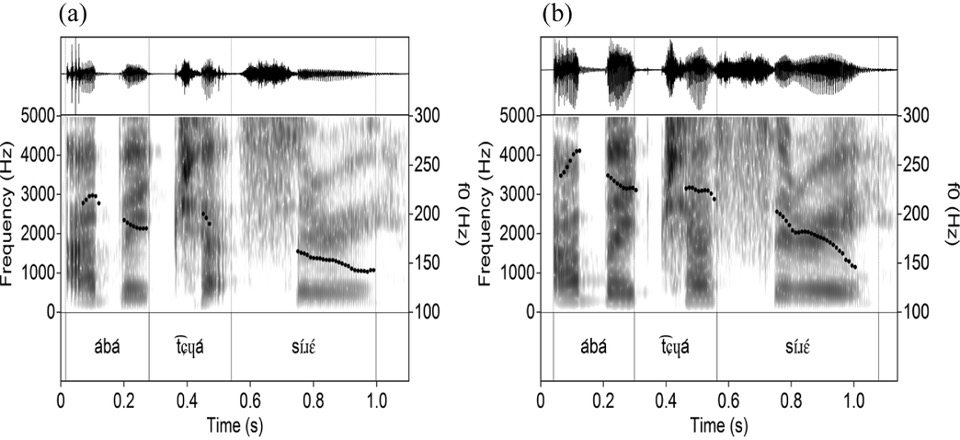
\includegraphics[width = 1\textwidth]{figures/akan.jpg}
	\caption{Waveforms and pitch curves of a declarative (right) and an interrogative by a female Akan speaker (Figure~7 in \textcite{genzel2020akan}) }\label{fig:akan}
\end{center}
\end{figure}

As shown in Figure~\ref{fig:akan}, the interrogative sentence is produced with a breathy voice quality at the end, as compared to the declarative sentence (F0 lowering here is a by-product of the laryngeal setting of producing the breathy voice). Table~\ref{tab:prosody:typology} lists some of the prosodic features that languages use to mark the differences between polar interrogatives and declaratives:



\begin{table}[H]
\begin{center}
\begin{tabular}{l|l}
\hline
Prosodic feature & Polar interrogative feature (language)\\
\hline \hline
Boundary tones: & H\% or LH\% (Dutch, French, Japanese) \\
 & HL\% (Roermond Dutch) \\
 & L\% (Catalan, Chickasaw, Bininj Gun-wok) \\
 \hline
Peak alignment & late peak alignment (Neapolitan Italian, Russian) \\
\hline
Peak height & Higher (Russian, Japanese) \\
\hline
Register expansion & Less downdrift (Wollof, Danish) \\
\hline
Final lengthening & Lengthening (Nateni) \\
\hline
Final voice quality & Breathy termination (Akan, Moba)\\
\hline
\end{tabular}
\end{center}
\label{tab:prosody:typology}
\caption{Intonational markings used to differentiate polar interrogatives and declaratives (adapted from \cite{butler2012typology})}

\end{table}%


Considering the fact that some languages do not use prosodic features for clause typing,\footnote{However, we do not have data on whether Vata or Shekgalagari uses prosody to distinguish imperatives from declaratives. Given the fact that languages tend not to have prosodic distinctions between declaratives and imperatives, our generalization has a good chance to hold.} it is possible that children do not have a priori knowledge that prosodic features are informative for clause type categorization. But what about speech acts? We do not have enough data from Vata to determine whether the question act could still carry a different set of prosodic features despite the fact that interrogatives are not marked by prosody, but given Gussenhoven and Chen's (\cite*{gussenhovenchen2000}) experiments with non-native prosodic contours, it is likely that speakers of Vata might be able to use rising intonation to identify questions. 

If children do not assume that prosody informs clause typing, Italian- and Portuguese-acquiring children might need to learn the connection between prosody and clause typing, in addition to learning clause type and speech act categories. But it is also possible that children do not need to learn this connection at all. If children assume that prosody informs speech acts, and that speech acts are informative of clause typing, prosodic information could indirectly help the learning of clause type categories. 

It is also possible that children come to the learning task assuming that prosody \tit{does} inform clause typing. For children learning languages like Vata, where prosody is irrelevant for clause typing in their language, the input might be such that this connection is simply uninformative. Thus, assuming a connection between clause typing and prosody would not make any difference for the learning the clause type categories. To test this possibility, we need to look at the input to Vata-acquiring children, and see if assuming the link between prosody and clause type would hinder children from learning the right clause type clustering. 

Another complication related to prosody is that languages use different prosodic features for clause typing, and many of them are not correlated with a rising F0 at the end. For example, Akan's breathy termination in fact results in the lowering of F0. Therefore, instead of having a built-in knowledge of the form ``final rise $\sim$ questionhood," children might need to learn which prosodic features are associated with which speech act/clause type clusters, the same way that they need to learn which morpho-syntactic features go with which clause type cluster.

Both English and Mandarin have dedicated morpho-syntactic features for interrogatives (e.g. subject-auxiliary inversion in English). But in both languages, it seems that there are also prosodic differences associated with interrogatives. We will discuss the prosodic features of these two languages in more details in Chapter~\ref{chap:man-cl} and Chapter~\ref{chap:prosody}.

\section{Acquisition of speech acts and clause types}
\label{sec:bg:acq}
\subsection{Early communicative abilities}
\label{sec:bg:acq:pre}
As mentioned in the previous chapter, it would be very useful for learners if they could rely on speech act information to learn how clause types are expressed in their language. Speech acts are, unfortunately, not directly observable, but there may be cues accessible to learners that are broadly indicative of speech act. One good candidate are cues for communicative intent.
Previous studies have shown that infants are sensitive to %can recognize
communicative intentions even in their first months of life, and they can distinguish signals for communication, such as eye contact, intentional pointing, and speech, from non-communicative signals. Infants tend to follow the gaze of their interactive partner. Newborn babies already show rudimentary form of gaze following (\cite{farroni2004gaze}); as young as 3 months of age, infants seem to automatically orient to gaze cues, as they could shift gaze fast with adult’s gaze direction (\cite{hood1998gaze}); 6-month-olds follow gazes that are communicative, such as adults' directly gazing at an object (\cite{gredeback2008gaze}), or being greeted (e.g. ``Hello!'') in infant-directed speech (\cite{senju2008gaze}). Human infants, but not chimpanzees, understand pointing as intentional (\cite{pika2006point, povinelli1997point,morissette1995joint}); 9-month-olds remember different aspect about an object depending on whether the object is presented in a communicative (such as pointing) vs.\ non-communicative scenario (\cite{yoon2008intent}); 12-month-olds not only follow the direction of pointing, but also infer that the pointing is to indicate information such as where a toy is hidden in hide-and-seek games (\cite{behne2005hide,behne2012point}). Starting from six months old, infants can readily interpret speech, but not other vocalizations like coughing, as indicating communicative intentions (\cite{vouloumanos2014intent}).

Of course, merely recognizing an act \emph{as communicative} is not the same as distinguishing speech acts -- beyond the recognition that there is communication, one needs to infer the function of the communication to approach speech act recognition.
Indeed, besides recognizing a signal as communicative, infants can attribute simple goals and desires to an agent, and use shared experience to infer their goals. By 9 months old, infants can recognize an agent's goal of reaching for an object (\cite{woodward1998goal,baldwin2001goal});\footnote{But studies show that still have difficulty with the avoidance type of goals until 14 months old (\cite{feiman2015goals}).} 14-month-olds can distinguish actions that are intentional and ones that are accidental, and only imitate actions that are intentional (\cite{carpenter1998intent,sakkalou2013goal}), and if things go wrong, they offer to help achieve others' goals (\cite{warneken2007goalrecog}); they could use shared experience such as cleaning up toys to interpret an agent's pointing as putting away the pointed object away, and would not attribute this goal to an agent who don't have the shared experience (\cite{liebal2009goal}).

Relatedly, it seems that infants have some understanding of other people's desires and beliefs, attitudes that are frequently associated with the speech acts of assertions, questions, and requests. For example, 9-months-old can distinguish whether someone is unwilling or unable to hand them a toy (\cite{behne2005goal}); 12-month-olds can use eye gaze and positive affect to infer which object an agent is going to reach for (\cite{phillips2002gaze}), and by 18 months old, infants use positive affect alone to infer which object the agent prefers, even if the preference is different from their own (\cite{repacholi1997desire}). Around 12 months old, infants can use pointing not to merely direct others' attention, but to request others to share information (\cite{kovacs2014request}); 13-month-olds seek information to clarify ambiguous situations (\cite{vaish2011request}); by 18 months old, infants are shown to be able to attribute beliefs to other people (\cite{onishi2005tom,surian2007tom,song2008earlytom,song2008false, scott2009tom,perner2012earlytom}, see \cite{scott2017review} for a recent review). 18-month-olds could use common ground knowledge shared with an agent to infer whether the agent is requesting an action with an object (e.g. open the door with the key) or simply playing with the object (\cite{schulze2015indirect}).%16-mo use pointing to solicit informaiton (\cite{begus2012point}); 2-year-olds are shown to use what others know when requesting help (\cite{oneill1996knowledge}). 
 


Infants also have some understanding of the norms of conversations. For example, from early on, they understand that conversations take turns. Longitudinal studies with 3 to 5-month-olds show that the overlap between infants' vocalization and parents' speech gradually decrease (\cite{hilbrink2013turn3mo}), and the rhythm of their vocalization starts to mimic the structure of a conversation, as they wait for parents to finish their turn (\cite{hilbrink2013turn,hilbrink2015,casillas2016corpus}); they also use turn transition points (e.g. questions) to cast predictive eye gaze to the next speaker (\cite{casillas2017turn}).

 
 %\textcite{} finds that 
 
In sum, this body of work suggests that by 18 months old, the communicative abilities needed to acquire the distinctions between speech acts and map them to clause types are in place. In the next section, we will see that indeed by this age, infants seem to figured out the major speech acts and are able to link them to their canonical clause types.



\subsection{Early knowledge of clause types and speech acts} \label{sec:bg:acq:spcl}

Previous studies show that children seem to have knowledge about clause types and the associated speech acts (in particular interrogatives and questions) from as early as 18 months old. 

Using corpus data, many studies show that infants can use one- and two-word utterances to express a variety of intentions that can be interpreted as \aqrs{} (\cite{bateson1975,bates1976language,ninio1994} among others); English-speaking children start producing interrogatives around 20 months starting with \twh-interrogatives (\citealt{tyack1977, stromswold1995, rowland2003cdswh}). From the comprehension side, results from corpus studies on parent-child interactions show that children begin to respond to parents’ questions, especially \tit{who, what, where} questions, appropriately around one and a half years old (\citealt{ervintripp1978, steffensen1978, shatz1978comprehension, shatz1978communicative, berningergarvey1981, shatzmccloskey1984, clark2015turn, moradlou2020} among others). 





Results from experimental studies show that around 12 months, English-speaking infants show sensitivity to differences in word order (\citealt{geffenmintz2015wordorder}) associated with declaratives and polar interrogatives. Data from preferential looking tasks show that already at 15 months old, infants look at the objects corresponding to the answers of \twh-interrogatives (\citealt{seidl2003wh, gagliardi2016wh, perkins2020filler}), though their success might not necessarily reflect knowledge of the syntax of \twh-interrogatives, as they might be relying on their knowledge of verb argument structure in the task (\citealt{perkins2019}). 

By 18 months old, infants seem to be able to distinguish questions from assertions, and use this distinction to infer the epistemic state of the speaker. \textcite{luchkina2018infant} test how well 18-month-olds’ learn labels of novel objects from speakers who made statements about familiar objects (e.g., \tit{This is a star}) and from speakers who asked questions (e.g., \tit{Is this a star?}). During the test phase, both types of speakers use statements to label a novel objects (\tit{Look, a lif! Lif!}). After repeating the statements several times, children are asked by an unfamiliar novel voice to look at one of the objects (e.g. \tit{Look, a lif! Where's the lif?}). They find that 18-month-olds only learn labels of objects from the speaker who made statements during the familiarization phase, but not from the question-askers. This result suggests that 18-month-olds can differentiate questions from statements, and furthermore, they can use this distinction to infer that question-askers might be a less reliable information source than statement-makers. 

\textcite{marshmallowqueen} demonstrate that 18-month-olds can associate interrogative syntax with the speech act of questioning with the preferential looking paradigm. In the experiment, infants watch a video of two puppets cheering a mechanical arm for delivering cookies into a box. During the test phase, one of the puppets leaves the scene while the cookie is being delivered, and is thus ignorant of whether there is a cookie in the box. Then participants either hear a polar interrogative \tit{is there a cookie in the box?} or a declarative \tit{there's a cookie in the box!} that could be uttered by either puppet. They find that at 18 months old, infants look more at the ignorant puppet when hearing the polar interrogative, suggesting that they understand the polar interrogative as a question uttered by the ignorant puppet.

\textcite{casillas2017turn} tap into children's knowledge of turn-taking to see if children differentiate questions from other types of speech acts. They measure how often children switch their gaze to track the upcoming speaker. Since questions are turn-transitioning points where a switch in speaker is mostly likely to happen, if children can identify questions, they should switch gazes to the upcoming speaker more often after questions. In the experiment, children are shown videos of a conversation between two puppets in one of four conditions: with normal speech, with words only (filtering out prosodic cues), with prosody, or with no speech. They find that even at 1 years old, children are faster at switching their gaze to the addressee after questions than non-questions in general. Breaking down the different cues to questions, they find that in the word-only condition, even 1-year-olds switch their gaze to the upcoming speaker more often after questions, but in the prosody-only condition, 5-year-olds still are at chance distinguishing questions from non-quesitons. These results suggest that 1-year-olds might be able to use the morpho-syntactic properties of interrogatives to infer questions. Similar results are replicated with 2.5-year-olds by \textcite{lammertink2015turn}.


As for imperatives and commands, \textcite{shipley1969} show that even in the ``telegraphic speech'' phase (15-30 months old), children respond appropriately to imperatives as commands. \textcite{orfitellihyams2012subj} show that 3-year-olds (and some 2.6-year-olds) can use the presence/absence of verb morphology to tell whether the sentence is a pro-drop declarative or an imperative, but it's possible that children in the experiments are using \tit{please} as a cue for command interpretation. 

Previous studies on questions in speech to children suggest that parents use questions in many different ways (\citealt{holzman1972, shatz1979, tamir1980, yu2019pedagogical}). In particular, compared to questions in adult-directed speech (\citealt{stivers2010}), parents tend to use question as a pedagogical strategy. \citealt{zaitsu2020} investigates the frequencies of the three basic clause types and the corresponding speech acts in speech to children between the age 1 to 3 from the Providence corpus (\citealt{ProvidenceCorpus}) of CHILDES (\citealt{CHILDES}). They find that although the three clause types generally are associated with their canonical speech acts, there are cases of mismatches (indirect speech acts). However these mismatches are often marked, and tend to form a systematic subcategory. For examples, when interrogatives are used as requests, we often see the presence of modals and attitude verbs in the sentence; when declaratives are used to perform questions, we often see rising prosody\footnote{Although they did not explicitly annotate the prosodic information; rising prosody is inferred from the use of question marks in the transcript.}. This is relevant because these systematic marking might alert the learners that these uses of the clause types may be somehow special. In particular, questions are often asked via rising declaratives, and requests made with interrogatives. 



Going beyond English and turning to Mandarin, we have less evidence for children's early knowledge of speech acts and clause types. Most study with younger children are documentations of their production data. Particularly, Mandarin-speaking children are observed to produce \ma-interrogatives, A-not-A interrogatives, and \twh-interrogatives before they turn 2 years old (\citealt{miao1986acq, miao1992, lee1989acq, litang1991int, lichen1997compprod, lichen1997comp, fan2012, lijingwong2017}). 

On the comprehension side, experimental studies testing children’s comprehension suggest that 18-30 month-olds can correctly link \twh-interrogatives to the question speech act, but are less likely to respond to A-not-A polar interrogatives (\textcite{moradlou2020}). However, this result might be due to the way the experiment is set up. During the experiment, children are asked polar interrogatives (e.g. \tit{Is this a duck?}) or \twh-interrogatives (e.g. \tit{What does a duck say?}) while looking at pictures of animals. But in this setting, particularly if the questioner is a person with authority, children might consider the polar question as redundant, and therefore tend to not respond to these questions. 

By 3 years old, Mandarin-children have adult-like interpretation of \twh-interrogatives (\citealt{fahn2003acq}), and that they can use prosodic information to determine whether the sentence is a \twh-interrogative or a declarative (\cite{WHanything}). In Mandarin sentences like  (\ref{bg-acq:negwh}) is ambiguous between a declarative and a \twh-interrogative. 

\bex{bg-acq:negwh}
\gll Xiaoyang mei	fang	\tun{shenme} shuiguo zai	xiangzili\\
Lamb \Neg{}	put	what		fruit		in	box\\
\trans a. ``What fruit didn't Lamb put in the box?''\\
b.	``Lamb didn't put any fruits in the box.''
\eex
In this case, the two interpretations are disambiguated by prosodic cues: assigning prosodic prominence on \tit{shenme} gives rise to a \twh-interrogative interpretation, and without prosodic prominence, the sentence is a declarative. \textcite{WHanything} show that 3-year-olds, like adults, can access both interpretations of the sentence.

\section{Summary}

In this chapter, I reviewed what we already know from the existing literature on the formal properties of clause types and speech acts and their analyses in the formal literature. Regardless of the theoretical approach, people agree on the three major clause types and their corresponding three major speech acts. 


Additionally, I reviewed literature on children's understanding of clause types and speech acts, and the linguistic and pragmatic capacities that they can draw from early in development, and what we know about the kinds of speech acts and clause types children are exposed to. The results from these studies suggest that by 18 months old, infants seem to have figured out the major clause types and speech acts, and the link in-between. These studies give us a developmental window for modeling the learning of clause types, namely that we need to take into account what infants know around 18 months old, to simulate how they figured out clause types and speech acts at this age. In the next chapter, I delve into the problem of how 18-month-olds figure out clause types. 





%In summary, children might face many challenges when learning interrogatives and their mapping to questions: English-speaking children should identify word order as a cue for interrogativity, but this information might be buried under many exceptions; Mandarin-speaking children should identify the markers for interrogativity (e.g.~\twh{}) despite some of these markers occurring in non-interrogative environments. Moreover, in both languages, children have to recognize the link between interrogativity and questionhood, which might be masked by exceptions in their input. So, how do children acquire interrogatives and their relationship to questions? In the next section, we will see that despite the noisiness of the input data, there is evidence suggesting that children nevertheless have adult-like understanding of interrogatives, questions, and their relationship at around three years old if not younger. 



 %\cite{evans2014ids} \cite{bernicot1987imp}

